%!TEX root = ../thesis.tex
%*******************************************************************************
%**************************** Introductory Chapter *****************************
%*******************************************************************************

\chapter{Introduction} %Title of first chapter
\label{chap:introduction}

\ifpdf
    \graphicspath{{Chapter0/Figs/Raster/}{Chapter0/Figs/PDF/}{Chapter0/Figs/}}
\else
    \graphicspath{{Chapter0/Figs/Vector/}{Chapter0/Figs/}}
\fi

%********************************** %First Section  **************************************
\section{Motivation}
Hominids have always manipulated and altered their environment. Ancient people replanted wild flora and helped drive various megafauna such as woolly mammoth and steppe bison to extinction \cite{Mann2015} \cite{Pushkina2008}. Today, we are still changing our surroundings, but at a historically unprecedented rate. Paul Crutzen popularised the term anthropocene in the early 2000s, defining it as the current geological period of Earth's existence, one where humanity has a significant impact on the planet's various systems, in many ways outcompeting natural processes \cite{Crutzen2006}. Our rapacious desire for resources has felled forests, excavated vast holes in the Earth, driven countless species extinct and burnt fossil fuels on a tremendous scale, releasing greenhouse gases (GHG) \nomenclature[z]{GHG}{Green House Gases} including carbon dioxide into the atmosphere. This last process has driven atmospheric CO$_{2}$ concentrations from 280ppm \nomenclature[z]{ppm}{parts per million} to 410ppm in two centuries \cite{NOAA2018}. The rate of accumulation is currently 2ppm and accelerating \cite{NOAA2018}. This accumulation of GHGs is driving climate change, leading to a near-surface temperature increase of 0.8\textdegree C since the start of the 20th century \cite{Hansen2010}. The consequences of the increased energy retained in the Earth system are many and varied. Sea levels have risen by 19cm in the same period \cite{Church2013}. Arctic sea ice coverage has decreased by $\approx 10.4\% \pm 1.7\%$ per decade in the last 30 years \cite{NSIDC2018}. The condition of the planet will undoubtedly continue to deteriorate in the coming decades. Continuing sea level rises will threaten tens of millions living at sea level in Bangladesh and Indonesia, amongst many other contries \cite{EJF2017}. Incidence of tropical diseases will worsen in equatorial regions and spread to the warming temperate zones \cite{Shuman2010}. Extreme precipitation events have already become more intense by 3.3\% and this trend is modelled to continue with a 5.2\% increase for each degree of warming \cite{Zhang2013}. Many of these conditions are now `baked-in' and will happen regardless of humanities efforts to avert them. This is because there is a lag between addition of GHG to the atmosphere and a new temperature equilibrium being reached of at least a decade \cite{Ricke2014}, but perhaps as much as a century for large GHG emissions \cite{Zickfeld2015}. Two degrees of atmospheric warming over pre-industrial temperature is now extremely likely, with four or more degrees a possibility \cite{IPCC2007}. We must now mitigate the risks posed by our changed and changing planet and act to prevent warming worse than two degrees, for the consequences of further increases are dire.

% Reference David McKay? Check his figures for consumption and correct if necessary
The main sources of GHG emission that humans are responsible for are combustion of fossil fuels for heat (industrial and domestic heating and cement production), transport (internal combustion engines and jet engines) and electricity production (typically with a boiler and steam turbine) and agriculture (deforestation and animals' methane production) \cite{MacKay2009}. We must rapidly reduce our GHG emission from current levels to near-zero or even negative rates \cite{MacKay2009}. In order to achieve this, heating, transport and electricity production must be decarbonised. Unfortunately, removing fossil fuels from heating and transport is most likely to be achieved with their electrification. This, coupled with a growing population and desire for increasing material living standards, means low-carbon electricity demand is going to dramatically increase in the near future. One study suggests the UK's annual electricity demand will grow from 340 to 423 TWh \cite{Bossmann2015}. 

%\cite{Zalasiewicz2017}

Low-carbon electricity production is currently produced from nuclear fission and renewables such as solar photovoltaic, solar thermal, wind, hydro, tidal, geothermal and biofuels. The acronym WWS (Wind, Water and Solar) \nomenclature[z]{WWS}{Wind, Water \& Solar} summarises the renewable methods with greatest potential for widespread adoption. 

While nuclear fission is very safe by the metric of energy produced per death caused \cite{Markandya2007} it has spawned several major accidents, suffers from issues of public acceptability, radioactive waste storage and, more recently, construction cost. Additionally, the current trend for an open fuel cycle where nuclear fuel is not reprocessed and then reused is wasteful. This practice drastically limits the potential of nuclear fission at scale, with current uranium reserves running out by the end of this century \cite{OECD2013}. WWS have tremendous potential and are currently gaining market share, with costs falling rapidly. For instance, some utilities are now bidding to supply electricity for as little as 3\textcent \: kWh$^{-1}$ \cite{IRENA2018}. For comparison, the Hinkley Point C nuclear fission plant will have a minimum supply price of 9.25p kWh$^{-1}$ \cite{NAO2017}. While some researchers have advocated for 100\% WWS by 2050 \cite{Jacobson2018} this seems unlikely with current energy storage technology as intermittancy is a significant problem for these technologies, specifically wind and solar \cite{Clack2017}. Much work is required to fully exploit their potential: drastic improvements in energy storage methods, a commensurate deployment of such technology, intelligent demand optimisation and improved distribution networks. Even then, it is unclear if WWS and/or nuclear fission could provide enough electricity for our future society. 

\section{Nuclear fusion}
A potential future alternative to both WWS and nuclear fission is nuclear fusion, the process of combining nuclei by which stars shine. Nuclear fusion power has several desirable attributes:

\begin{itemize}
  \item Low CO\textsubscript{2} emissions
  \item High fuel energy density (reduced resource extraction burden)
  \item Abundant fuel (or feedstock for the manufacture of fuel)
  \item Dispatchable power generation
  \item No criticality (runaway) risk, unlike nuclear fission power
  \item High plant power density (GW scale facilities on the order of 1 km\textsuperscript{2}). 
\end{itemize}

However, to date the goal of electricity generation from nuclear fusion has eluded scientists and engineers.  

\subsection{Discovery}
Einstein's energy-mass equivalence, $E=mc^{2}$ led Arthur Eddington to hypothesise that the energy released by the sun was through the fusion of hydrogen nuclei into helium nuclei. However, contemporary predictions of the temperature required for the sun's power output did not match observations. Indeed, the temperatures observed seemed too low for nuclei to overcome the Coulomb energy barrier - the repulsive force experienced by two nuclei. The development of a theory of quantum tunnelling in the late 1920s by Gamow and others, predicted thermonuclear temperatures in accordance with observations of the sun and resolved the problem of stellar temperatures.

In the 1930s Mark Oliphant, Paul Harteck and Ernest Rutherford conducted particle beam experiments, bombarding various targets with deuterons. After several less interesting combinations, they observed ``on bombarding heavy hydrogen with diplons\footnote{Diplon was a contemporary name for what we now call a deuteron.} an enormous effect was produced'' \cite{oliphant1934}. This included the emission of high energy neutrons. Soon thereafter, plans for fusion weapons and controlled fusion power were developed.

%https://www.chemteam.info/Chem-History/Rutherford-1934b/Rutherford-1934b.html

\subsection{Possible reactions to harness}
Trying to fuse nuclei is difficult, as scattering via the Coulomb force is far more likely than fusion for all potential reactants. This Coulomb barrier is proportional to the product of the charges of the reactants as shown in equation \ref{eq:coulomb}, where $k_{e}$ is the Coulomb constant, $Z_{i}$ the respective atomic numbers, $e$ the charge on the electron and $r$, the interaction radius.

\begin{equation}
  \label{eq:coulomb}
  U_{coul} = k_{e}\frac{Z_{1}Z_{2}e^{2}}{r}
\end{equation}

Given this, it is only plausible to employ light nuclei for energy production. Of the light nuclei, certain reactions are more likely than others, with a greater cross-section for a given collision energy. They are shown in table \ref{tab:fuels} below.

\begin{table}[H]
  \centering
  \begin{tabu} to \textwidth {X X X X X}
    \toprule
    Fuel          & Products          & Q-value (MeV) & $\sigma \mathrm{(10 keV) (barn)}$ & $\sigma \mathrm{(100 keV) (barn)}$ \\
    \midrule
    D + T         & $\alpha$ + n        & 17.6          & $2.72\times10^{-2}$    & 3.43                    \\
    D + D         & T + p             & 4.04          & $2.81\times10^{-4}$    & $3.3\times10^{-2}$      \\
    D + D         & $^{3}$He + n      & 3.27          & $2.78\times10^{-4}$    & $3.7\times10^{-2}$      \\
    D + $^{3}$He  & $\alpha$ + p        & 18.3          & $2.2\times10^{-7}$     & 0.1                     \\
    p + $^{11}$B  & $3\alpha$           & 8.68          & $4.6\times10^{-17}$    & $3\times10^{-4}$        \\
    \bottomrule
  \end{tabu}
  \caption{Comparison of potential fusion fuels. The Q-value is the combined kinetic energy of the reaction products. $\sigma$(E) is the cross-section of the reaction at a given energy, E, with centre-of-mass energies.}
  \label{tab:fuels}
\end{table}

At an energy of 10 keV \nomenclature[z]{keV}{kilo electron-Volt} the D-T fusion reaction has a likelihood 100-fold of the next easiest reactions. It also has a large Q-value, with 17.6 MeV of binding energy released by the reconfiguration of the fuel nucleons. This energy is split between the products such that they have equal momentum, with the $\alpha$-particle receiving $\frac{17.6}{5} \mathrm{MeV} = 3.5 \mathrm{MeV}$ and the neutron the remaining 14.1 MeV. D-$^{3}$He and p-$^{11}$B fuels are aneutronic, with only charged products. These fuels would obviate several difficult problems associated with D-T fusion which arise from the energetic emitted neutrons. The principal benefit would be a reduced burden on materials science to develop radiation tolerant structural and plasma facing materials, qualified in time for usage in a reactor. There would also be a significant reduction in the quantity of radioactive waste generated, compared with a D-T fuelled reactor. Unfortunately, aneutronic fuels require extraordinary temperatures to fuse, far beyond anything achieved to date, or conceived as possible in a tokamak in the near future. D-T fuel is currently envisioned as the fuel mixture for nearly all government sponsored research programmes. Some private efforts are attempting to use other fuels, especially those aforementioned aneutronic reactions \cite{TAE2018}.

\subsection{Development}
The 1950s saw the invention and development of so-called `pinch` fusion concepts. As a current flows through a tube of conducting medium (such as a plasma) the magnetic field generated acts in tandem with the current to crush the material to a filament by a Lorentz, or $\mathbf{j \times B}$ force. This is a kind of confinement, momentarily holding plasma ions in an increased density state. By bending a tube into a toroidal shape, matter might be circulated about a device, permanently confined. In reality, the gradient of the electric field across the torus acts to break confinement and lose material. The pinch concept was developed by Soviet scientists Sakharov and Tamm, into the tokamak. This was similar to previous designs of toroidal pinch machines, such as the British ZETA, \nomenclature[z]{ZETA}{Zero Energy Thermonuclear Assembly} but the relative strength of fields was different. Rather than having the dominant field be produced by the plasma current, in a tokamak the dominant field is generated by the toroidal field coils which wrap around the toroidal plasma chamber. Over the coming decades this would prove to be a more stable confinement system than other approaches. 

Throughout the rest of the 20th century, the tokamak concept came to dominate magnetic confinement fusion research. Plasma physicists around the world continued to design devices and plasma scenarios which attempt to avoid plasma instabilities and maximise the plasma triple product, developed from Lawson's criterion \cite{lawson1955}. The triple product, $nT\tau_{E}$, is the product of the plasma density, temperature and energy confinement time, respectively. Figure \ref{fig:triple_product} shows a plot of this performance metric against time. One can see the progress in relation to the well known Moore's Law in computing performance per unit cost and the beam energy of various particle colliders. Viewed in this way, fusion power has achieved remarkable progress across the decades (logarithmic and temporal).

\begin{figure}
%  \figuretitle{}
  \centering
  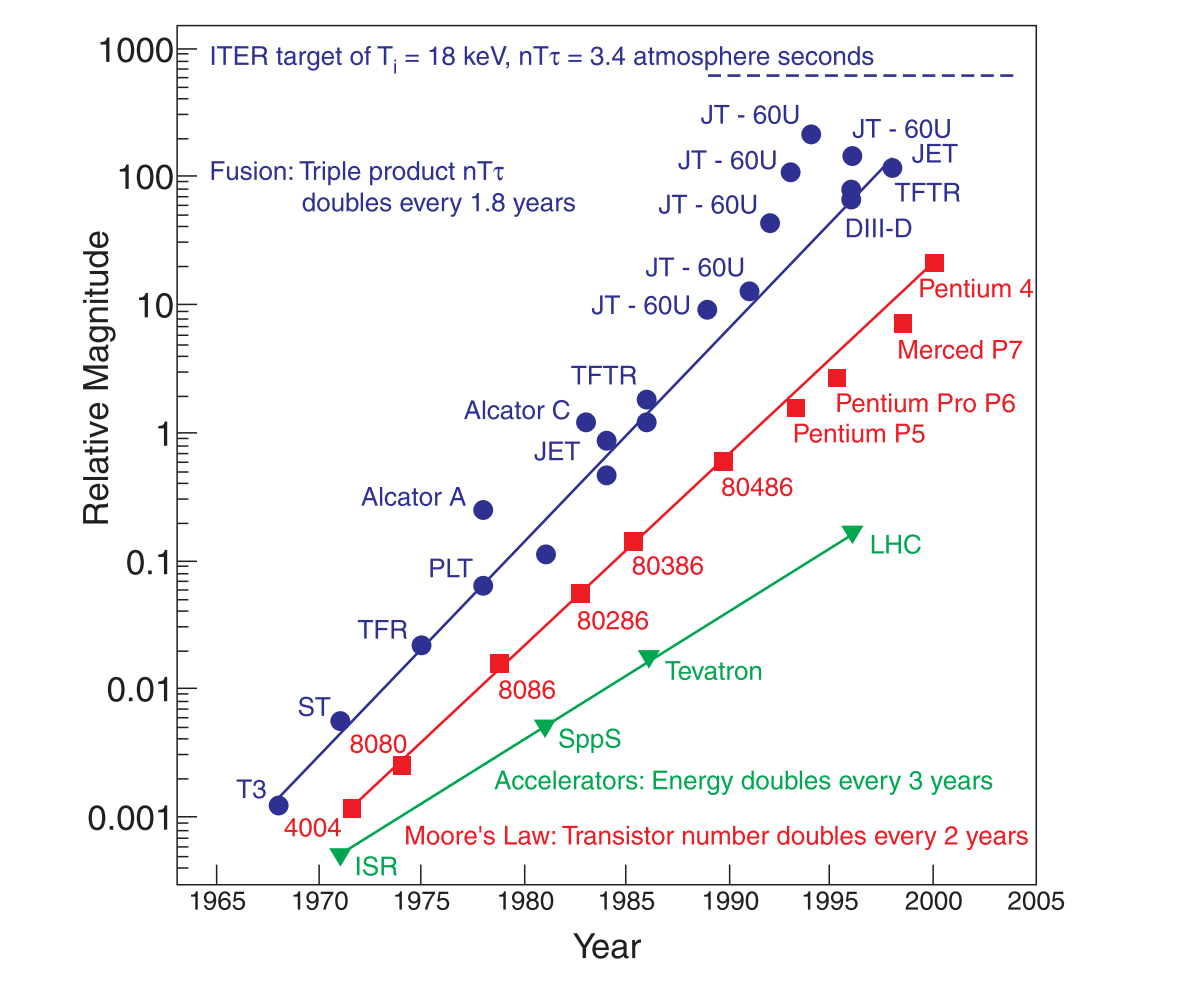
\includegraphics[width=0.7\textwidth]{triple_product.png}
  \caption{Fusion triple product achieved plotted against time. Similar progress measures for computing and particle physics are also shown. Figure from \cite{Yamada2012}.}
  \label{fig:triple_product}
\end{figure}

\subsection{Future plans}
There are many aspects of nuclear fusion power which require significant work before an electricity producing reactor could be constructed. In the field of plasma physics these include, improving energy and particle confinement, quelling various powerful emissions from the plasma (disruptions, ELMs, fast ions, runaway electrons) and increasing plasma temperatures. The ITER \nomenclature[z]{ITER}{International Thermonuclear Experimental Reactor} reactor under construction in the south of France will provide a test for plasma physics knowledge, through the equilibrium operation of a `burning' plasma. However, the plasma `core' is only one aspect of a functioning fusion reactor. The surrounding systems of an electricity producing reactor necessarily include:

\begin{itemize}
  \item Fuelling by gas or pellet injection
  \item Diagnostics to determine the state of the plasma and the plant
  \item Heating systems including micro and radiowaves and energetic particle beams
  \item Plasma heat and particle exhaust (divertor)
  \item Blanket for fuel breeding and capture of neutron energy
  \item Electricity production with heat exchangers, gas turbines and generators
  \item Tritium extraction, storage and recycling
  \item Cryoplant for the cooling of magnetic coils and other systems
  \item Remote handling for the maintenance of the other systems
\end{itemize}

While ITER will advance our understanding and experience of several of these ancillary systems, additional devices will be required before fusion electricity can be realised. These might include one or several demonstration reactors. Progress is crucial in materials science, as the systems listed above must operate for years without being degraded by plasma etching, radiation damage and stresses induced by extreme temperature gradients. Consequently, it is commonly held that a device for the production of 14.1 MeV \nomenclature[z]{MeV}{mega electron-Volt} neutrons at a useful flux is also required for the development and testing of radiation tolerant materials.

\section{Radiation-matter interactions}
Nuclear fusion gives rise to various energetic particles. The neutrons are emitted with $\frac{4}{5}$ of the total energy liberated, to give 14.1 MeV of kinetic energy. Photons are constantly generated in a tokamak plasma. Low energy photons are created through the excitation and de-excitation of atomic electrons, while Bremsstrahlung radiation arises from the acceleration of charged particles. This mixed radiation field is then further complicated by numerous interaction process, as neutrons and photons from the plasma interact with the device. What follows is a short primer on the possible interaction processes for the principle particles, the neutron and photon.

\subsection{Neutron}
The neutron is a sub-atomic particle of mass $1.674927471(21)\times10^{-27}$kg \cite{NIST2018}, composed of three quarks. It can exist as part of a nucleus or unbound, where it has a mean lifetime of $877.7 \pm 0.7$s \cite{Pattie2018}. While it is itself uncharged it can produce ionising radiation through interactions with other matter. These reactions are via the strong, weak, graviational and electromagnetic\footnote{While the neutron has zero electric charge, it does have a magnetic moment, and is therefore acted upon by electromagnetic fields.} forces. When neutrons undergo collisions with nuclei, the ensuing process is strongly dependent on the combined energy of the reactants. The neutron-matter interaction processes of interest for this work are outlined below.

\subsubsection{Elastic scattering}
\label{subsubsec:elastic}
Neutrons can scatter off nuclei. In the context of fusion neutronics an elastic scattering event is defined as a neutron-nucleus reaction where no kinetic energy is transferred into excitation of the nucleus. Both the kinetic energy and momentum of the reactants are conserved. Although scattering is a quantum-mechanical phenomenon, properly described by the interacting wave functions, in this case a `billiard ball' treatment satisfactorily describes reactions. 

The fast fusion ($> 1 \mathrm{MeV}$) neutrons are significantly more energetic than the nuclei in condensed matter ($\approx 1 \mathrm{eV}$), as such, the target nuclei may be thought of as at rest. In elastic scattering the energy lost by an incident neutron is gained by the target nucleus. The energy transferred is a function of the target nucleus mass, as shown below.

\begin{equation}
  \frac{1}{2}m_{n}v_{n,i}^{2} = \frac{1}{2}m_{n}v_{n,f}^{2} + \frac{1}{2}m_{a}v_{a,f}^{2}
  \label{eq:conserve_energy}
\end{equation}

Where $m_{n}$ is the mass of the neutron, $m_{a}$ the mass of the target nucleus, $v_{n,i}$ is the initial velocity of the neutron, $v_{n,f}$ the final velocity of the neutron and $v_{a,f}$ the final velocity of the nucleus. Conservation of momentum can be written as below.

% Conservation of energy, equation \ref{eq:conserve_energy} may be rewritten as the following.
%
% \begin{equation}
% %  v_{n,i}^{2} - v_{n,f}^{2} = \frac{m_{a}}{m_{n}}v_{a,f}^{2}
%   (v_{n,i} - v_{n,f})(v_{n,i} + v_{n,f}) = \frac{m_{a}}{m_{n}}v_{a,f}^{2}
%   \label{eq:conserve_energy_2}
% \end{equation}
%
% Given conservation of momentum the below also applies.
%

\begin{equation}
  m_{n}v_{n,i} = m_{a}v_{a,f} - m_{n}v_{n,f}
  \label{eq:conserve_momentum}
\end{equation}

With equations \ref{eq:conserve_energy} and \ref{eq:conserve_momentum} one can derive a quantity known as $\alpha$, the fraction of the initial energy retained by a neutron in a head on collision, as a function of target nucleus mass, A. For the derivation see \cite{harms1975}. The expression for $\alpha$ is as follows.

\begin{equation}
  \alpha(A) = \left(\frac{1-A}{1+A}\right)^2
  \label{eq:alpha}
\end{equation}

One can see that lighter nuclei, of closer mass to neutrons more effectively moderate the energy of neutrons. A collision with a single proton will halt the incident neutron, $\alpha(1) = 0$. Heavier nuclei such as $^{186}$W give $\alpha(186) = 0.9787$ so scattered neutrons retain almost all of their energy.

%
% Equivalently expressed as the following.
%
% \begin{equation}
%   v_{n,i} + v_{n,f} = \frac{m_{a}}{m_{n}}v_{a,f}
%   \label{eq:conserve_momentum_2}
% \end{equation}
%
% Dividing equation \ref{eq:conserve_energy_2} by equation \ref{eq:conserve_momentum_2} results in the speed of the nucleus after the collision.
%
% \begin{equation}
%   v_{a,f} = v_{n,i} - v{n,f}
%   \label{}
% \end{equation}

\subsubsection{Nuclear reactions}
\label{sec:nuclear_reactions}
Nuclear reactions are distinct from elastic scattering. Rather than solely redistributing energy and momentum, reactions reconfigure nuclei and create new particles. There are two principle ways this can happen:

\begin{itemize}
  \item Direct nuclear reactions - a single nucleon in the target particle interacts with the incident particle. The interaction time is very limited, around $10^{-21}\mathrm{s}$ (i.e. the incident energy is high). Direct reaction products are anisotropically distributed, typically forward focused.
  \item Compound nucleus reactions - many nucleons interact together over a greater period of time, perhaps $10^{-18} - 10^{-16}\mathrm{s}$. The incident particle and the target nucleus coalesce into a new, excited nucleus. The collection of nucleons within the nucleus reach thermal equilibrium after a series of collisions. At some point, the excited compound nucleus will decay, but the mode of decay will not depend on the method of compound nucleus formation. Instead, the decay mode, or `exit channel' is dependent on the compound nucleus excitation energy and various nucleus-specific probabilities. 
\end{itemize} 

This dichotomy is not entirely accurate, as the incident particle always affects multiple nucleons, but for so-called direct nuclear reactions, this is minor. Reactions can also be exothermic or endothermic, liberating or requiring energy to occur, respectively. This is recorded by the `Q-value' of a given reaction, say $^{208}$Pb(n,2n)$^{209}$Pb, where Q = -7.37 MeV. This neutron multiplying reaction is endothermic and requires an energy input to occur. A plot of cross-section against energy will clearly show this `threshold' behaviour, with zero probability of reaction until the minimum input energy is achieved. Exothermic reactions, by contrast can occur at any energy.

% I need something on compound nuclei as resonances. Interaction cross-sections should have been introduced prior to this.

\paragraph{Inelastic scattering}
An inelastic neutron scatter involves the target nucleus absorbing the incident neutron, forming an excited, compound nucleus and then re-emitting the neutron. The nucleus remains excited and emits a gamma ray to dissipate excess energy and reach its ground state. Given this and radiative capture, neutron fields usually beget gamma fields.

\paragraph{Radiative capture}
Radiative capture is similar to inelastic scattering, with an incident neutron also forming an excited compound nucleus. However, here a neutron is not re-emitted, only a gamma ray. This reaction is more likely at lower energies, given the slower relative velocity of reactants and therefore longer period for interaction. The reaction acts as a neutron `sink', removing neutrons from the system and is therefore an essential component of neutron shielding, along with moderating material and gamma-shielding.

\paragraph{Fission}
Inter-nucleon nuclear forces hold nucleons together in a spherical nucleus. With the addition of an extra nucleon (and its kinetic energy), this attraction can be overcome, distorting the nucleus into a dumbell shape, with two lobes. Sufficient energy will mean these lobes repel beyond the point of no return. As the electrostatic repulsion of the positively charged particles becomes greater in magnitude than the attractive nuclear force, the nucleus is fissioned. Nuclear fission is not normally associated with nuclear fusion reactors, however the fissioning of lithium to produce tritium fuel in breeder blankets is an important process for the viability of fusion as an energy source. Also, uranium is present in beryllium containing ores and even after refining, some remains as an impurity. One variant of the proposed European fusion reactor design, DEMO, is set to contain 560 t of beryllium. At 30 wppm uranium concentration (the ITER requirement) this results in 17 kg of uranium \cite{kolbasov2016}. A small amount is fissile as $^{235}$U, while the remaining $^{238}$U is fissionable by high energy neutrons. The daughter nuclei from actinide fission and bred transuranics will undoubtedly complicate the process of reactor component recycling \cite{cambi2010}.

\paragraph{Multiplication}
An incident neutron can result in multiple neutrons being emitted, a so-called multiplication reaction, (n,2n), (n,3n), etc. the reaction is always endothermic. Multiplication reactions are important in the context of tritium breeding in nuclear fusion blankets, increasing the neutron flux and therefore the production of tritium. Higher yield multiplication reactions have a greater energy requirement and thus a higher energy threshold. Materials such as beryllium and lead have high multiplication cross-sections, with beryllium having the lowest energy threshold for (n,2n) by some margin at approximately 2.7 MeV.

\subsection{Photon}
The photon is an elementary particle, indivisible by nature. Aggregated, photons provide one way of conceptualising an electromagnetic field. Photons travel in a vacuum at 299,792,458 ms$^{-1}$ and are created by various processes, across a wide spectrum of energies. The sources inside a fusion reactor include various plasma processes, neutron-matter interactions and radioactive decay amongst others. 

\subsubsection{Radioactive decay}
The gamma ray, or gamma photon, is a photon emitted by a nucleus. They can have energies from several keV to many MeV, overlapping in energy with X-rays\footnote{X-rays are produced by interactions with and between electrons. These processes include bremsstrahlung radiation, or X-ray fluorescence. Aside from an arbitrary energy and associated wavelength distinction, gamma photons and X-ray photons cannot be distinguished without knowledge of their source.} The gamma ray is emitted from an excited nucleus, often preceded by $\alpha$ or $\beta$ decay. As stated in section \ref{sec:nuclear_reactions} gamma emission also occurs as a result of compound nucleus formation during radiative capture and inelastic scattering. Gamma photons are ionising radiation and thus biologically hazardous. 

\subsubsection{Bremsstrahlung}
Literally `braking radiation', bremsstrahlung is the process whereby photons are generated as a charged particle is decelerated. As the braking particle is slowed, the kinetic energy lost is conserved to become a new photon. The energy spectrum of the emitted photons is continuous and will move to higher frequencies as the bombarding particle energy is increased. Bremsstrahlung is an important process in the plasma physics of nuclear fusion power. Unfortunately, Coulomb scattering is significantly more likely than fusion and these ion-ion and especially electron-ion scattering events generate significant bremsstrahlung radiation, slowing the potential reactants and dissipating energy from the plasma. The expression for bremsstrahlung power loss in a plasma is given as equation \ref{eq:bremsstrahlung}. 

\begin{equation}
  \label{eq:bremsstrahlung}
  P_{b} \propto T_{e}^{\frac{1}{2}} n_{e} \sum_{i} n_{i} <Z_{i}>^{2}
\end{equation}

It can be seen that the power is proportional to the square root of the electron temperature and the square of the average ion charge state \cite{schuster2017}. The latter relationship is one reason why so-called `advanced' fusion fuels such as p-$^{11}$B are so much more difficult to fuse than purely hydrogenous fuels \cite{rider1995}.

\subsubsection{Photoelectric}
The photoelectric effect is the phenomenon where incident photons are absorbed by atomic electrons and the electron is rapidly dislodged from the atoms electrostatic attraction. The energy threshold for the ejection of the most loosely bound electrons is known as the element's work function and is typically in the range 2--6 eV. It is in this low energy range where the photoelectric effect is most prevalent. An incident photon's energy can be described as $E=h\nu$ where $h$ is Planck's constant and $\nu$ is the photon frequency. If this energy is smaller in magnitude than the work function, no electron emission is observed, regardless of the photon flux. Larger incident photon energies can eject more tightly bound electrons, where energies in the MeV range may be required for photoelectric emission in some elements. The photoelectric effect is a major mechanism for the absorption and therefore `sinking' of photons.

\subsubsection{Compton scattering}
\label{subsubsec:compton}
Compton scattering is a mid-energy range photon-matter interaction between photons and charged particles. Incident photons lose energy, transferring it to the recoiling charged particle, usually an electron. The reduced photon energy corresponds with an increase in photon wavelength. The relationship between initial and final wavelength and scattering angle is shown as equation \ref{eq:compton_scattering}, where $\lambda$ is the initial wavelength, $\lambda'$ is the scattered wavelength, $h$ is Planck's constant, $m_{e}$ the mass of the electron and $\theta$ the scatter angle.

\begin{equation}
  \label{eq:compton_scattering}
  \lambda' - \lambda = \frac{h}{m_{e}c}(1-cos\theta)
\end{equation}

\subsubsection{Pair production}
Pair production is the general term for the creation of a particle and its antiparticle from an electrically neutral boson. In the context of photon interactions it is typically understood as the creation of an electron and positron from an energetic photon i.e., $\gamma \rightarrow e^- + e^+$. The photon is destroyed in the interaction. The particles are created from the incoming photon energy, which therefore must be at least equal to the rest mass of the particle pair, $2 \times 0.511 \mathrm{MeV} = 1.022 \mathrm{MeV}$. The process is the dominant high-energy photon-matter interaction. 

\section{Nuclear data}
Nuclear data (ND) is the general term for nuclear physics quantified and recorded for later retrieval. The behaviour of nuclei, in particular when under bombardment by nucleons and light nuclei can be probed by a variety of experiments. These typically utilise monoenergetic beams of particles and arrays of detectors to determine reaction likelihood (cross-section) and information on the reaction products (emitted energy \& angle). These experiments are then repeated through the energy spectrum, from meV to the MeV range. Once experimental nuclear interaction findings are generated, they are typically submitted to and stored in the EXFOR database. This is a publically queryable dataset of experiments to date. While the EXFOR dataset covers many nuclides, reaction channels and energies, this parameter space is very large and expensive to explore with nuclear physics experiments. In some instances, for example with short-lived radioisotopes such as metastables, it is not possible to peform the appropriate experiment. In this case, any exant experimental data is augmented with information derived from theoretical nuclear physics models. These data, from experiment and theory are used to develop or `evaluate' a bundle of nuclear data typically grouped by incident projectile and target nuclide. The evaluated files include likelihoods of interaction for various reactants (cross-sections) but also reaction product energy spectra, angular distributions, decay data, uncertainty information and more. There is a globally standard format known as Evaluated Nuclear Data File (ENDF) \nomenclature[z]{ENDF}{Evaluated Nuclear Data File} which specifies the scope, layout and precision of these files. The current version of the ENDF format is ENDF-6 \cite{Herman2010}. As well as the reaction information listed above and detailed below, the files also contain information on contributing experiments and modifications which occurred during data evaluation. There are a series of different nuclear data libraries which constitute different attempts to capture and record the nuclear behaviour of a variety of nuclides. These may be general purpose (e.g. JENDL \cite{shibata2011}, \nomenclature[z]{JENDL}{Japanese Evaluated Nuclear Data Library} TENDL \cite{Rochman2016} \nomenclature[z]{TENDL}{TALYS-based Evalulated Nuclear Data Library} and the confusingly named ENDF/B \cite{brown2018}\nomenclature[z]{ENDF/B}{Evalulated Nuclear Data File B}) or more specialist (e.g. EAF\cite{packer2011} \nomenclature[z]{EAF}{European Activation File}). Many countries with nuclear programmes have developed their own nuclear data libraries over time. 

ENDF type files are typically stored as ASCII \nomenclature[z]{ASCII}{American Standard Code for Information Interchange} text. They are arranged hierarchically as displayed in figure~\ref{fig:endf}. The MAT or material is typically but not exclusively a nuclide, it can also be elemental or even compound in nature. A MAT code is a unique reference for a material, such as 125 for \textsuperscript{1}H or 7443 for \textsuperscript{186}W. Each material contains several `files' referred to by an MF number. These contain the data listed in the sections below. Each MF, or file, is split into MTs. 

\begin{figure}[ht]
%  \figuretitle{}
  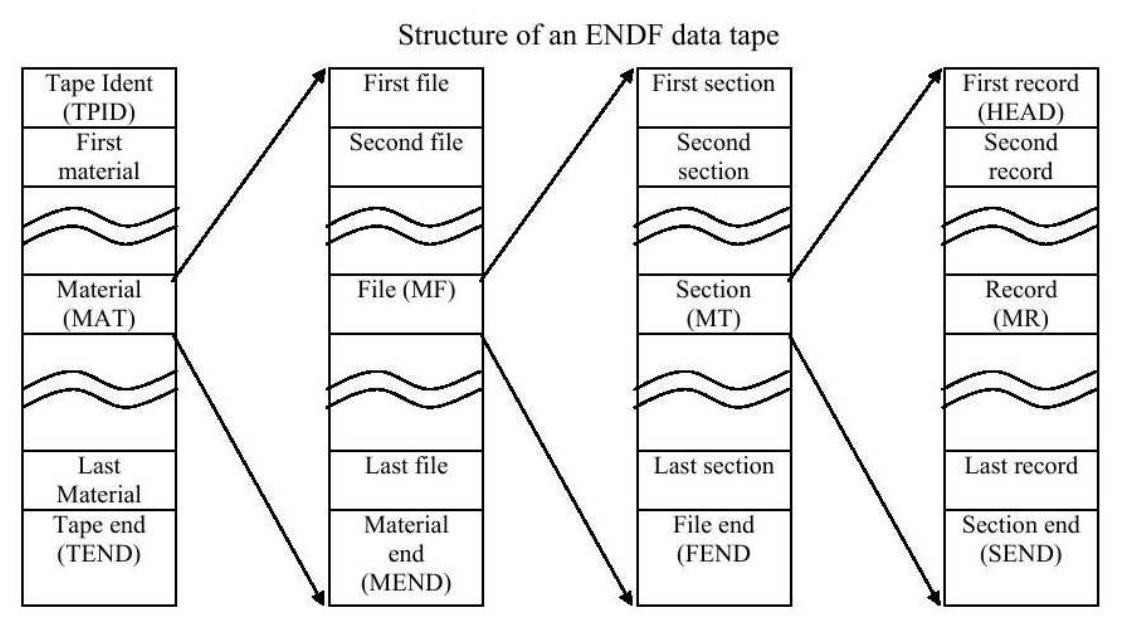
\includegraphics[width=\textwidth]{endf_architecture}
  \caption{The layout of an ENDF `tape', containing materials (typically only one material per tape), which contain files, which contain sections, which contain records.}
  \label{fig:endf}
\end{figure}

Nuclear data `processing' is required to turn the contents of an ENDF formatted file into a form that radiation transport and activation-transmutation codes can use. This is accomplished with codes such as NJOY \cite{MacFarlane2010} or PREPRO \cite{cullen2017}. These takes ENDF type files and process the wealth of information present, discarding some, performing various types of interpolation on others, etc. The resulting processed files, of use to nuclear analysts and other end users, are explained in chapter~\ref{chap:group_structure}, section~\ref{subsec:nd_processing}.

% \begin{itemize}
%   \item PENDF (Point-wise ENDF) is an intermediate file type, generated principally by reconstructing and broadening resonance parameters.
%   \item ACE (A Compact ENDF) is a machine readable file for stochastic radiation transport codes such as MCNP. 
%   \item GENDF (Group-wise ENDF) is MG (Multi-Group) nuclear data, required as input for deterministic codes and activation-transmutation programmes.
%   \item Probability tables (PTs) distributions of possible resonances for the URR (Unresolved Resonance Range).
%   \item Self-shielding factors (SSFs) are an estimated factor between a `true' reaction rate depressed by neutron absorption and an erroneously calculated one. They are essential for the correct calculation of RR (Reaction Rates) in systems with a neutron population in the resonant and thermal regions.
% \end{itemize}

A brief introduction to the nuclear physics encoded in ENDF type data and its various uses are given below.

\subsection{Resonance parameters}
The cross-section as a function of interaction energy is often an irregular, unsmooth shape due to the presence of nuclear resonances. These resonances are compound nuclei. That is, compound nuclear reactions where a short lived particle, a compound nucleus is temporarily formed. These nuclear resonances occur because the nucleus is a quantum mechanical system, with certain, discrete energy levels permitted. Methods for predicting nuclear reactions based on forces within the nucleus remain a work in progress as the inter-nucleon forces inside the nucleus are too complex to currently model, especially for larger nuclei. Insights can however still be gained from `black-box' models of the nucleus, where internal understanding is not assumed. One such approach is the R-Matrix interaction framework. In this method, unknown internal properties are parameters which can be deduced by comparison with experimental results. This method can be performed to varying degrees of complexity, with or without particle spin dependence, multiple reaction channels, etc. Other resonance formalisms are typically simplifications of the R-Matrix approach.

Rather than trying to record the cross-section for all interaction energies in a tabulated way, it is easier to reconstruct cross-sections from some `background' ($\sigma$, E) tuples and a series of summed resonance curves parameterised by resonance theory. These curves have a functional description, dependent on energy with various parameters determining their shape. A simple Breit-Wigner distribution is shown as equation~\ref{eq:breit-wigner}. This form is appropriate for non-overlapping resonances. The more sophisticated R-Matrix approach is required with overlapping resonances. 

\begin{equation}
  \sigma(E) =  \frac{\pi\lambdabar^{2}(2J + 1)}{(2s_{n} + 1)(2s_{t} + 1)}  \frac{\Gamma_{i}\Gamma_{f}}{[(E-E_{r})^{2} + \Gamma^{2}_{t}/4]} dE
  \label{eq:breit-wigner}
\end{equation}

Where $E$ is centre-of-mass energy of the system, $\Gamma_{i}$ is the partial resonance width to decay to the initial state, $\Gamma_{f}$ is the partial width to decay to the final state, $\Gamma_{t}$ is the total width, $\lambdabar$ the reduced particle wavelength, $E_{r}$ the rest mass energy of the resonance, $J$ the resonance total angular momentum, $s_{n}$ the neutron spin and $s_{t}$ the target spin \cite{Libby2005}. The $\Gamma$ values, or widths, are inversely related to the stability of the resonant nucleus, those with a very narrow width will correspondingly exist for longer before decay than those with very large widths.

The shape of resonance peaks in the interaction likelihood and energy space is a function of temperature. This is best explained by considering a monoenergetic neutron flux incident on a block of material. Despite the flux beam being monoenergetic in the lab frame, the neutron-nucleus interactions have a distribution of energies. This is dependent on the temperature of this material (higher temperatures act to widen the spread of interaction energies). As such, resonances are Doppler broadened as material temperature increases. An advantage of reconstructing cross-sections from resonance parameters is that the temperature dependence of cross-sections can be handled in an elegant and flexible way. 

While resonances at lower energies are detectable by experimental methods, at higher energies it becomes difficult to distinguish between neighbouring resonances. This is because the average spacing between nuclear levels, $\left<D\right>$, decreases with energy while the average resonance width, $\left<\Gamma\right>$, increases. Where $\left<D\right> \approx \left<\Gamma\right>$ there exist bunches of partially overlapping resonant cross-section peaks. This is the transition from the Resolved Resonance Range (RRR) to the Unresolved Resonance Range (URR). An overview of the cross-section from thermal to MeV energies for a heavy nucleus is shown as figure~\ref{fig:au-197_sigma_tot}. Resonances in the URR region are still important for self-shielding effects (see chapter~\ref{chap:group_structure}). While no experimental data is available on the precise resonance locations in the URR, average level widths and spacings are given in the appropriate ND. This average approach can be improved on with so-called probability tables. Resonance parameters are stored within the MF=2 file of an ENDF formatted entry. 

\nomenclature[z]{RRR}{Resolved Resonance Range}
\nomenclature[z]{URR}{Unresolved Resonance Range}

\begin{figure}[ht]
%  \figuretitle{}
  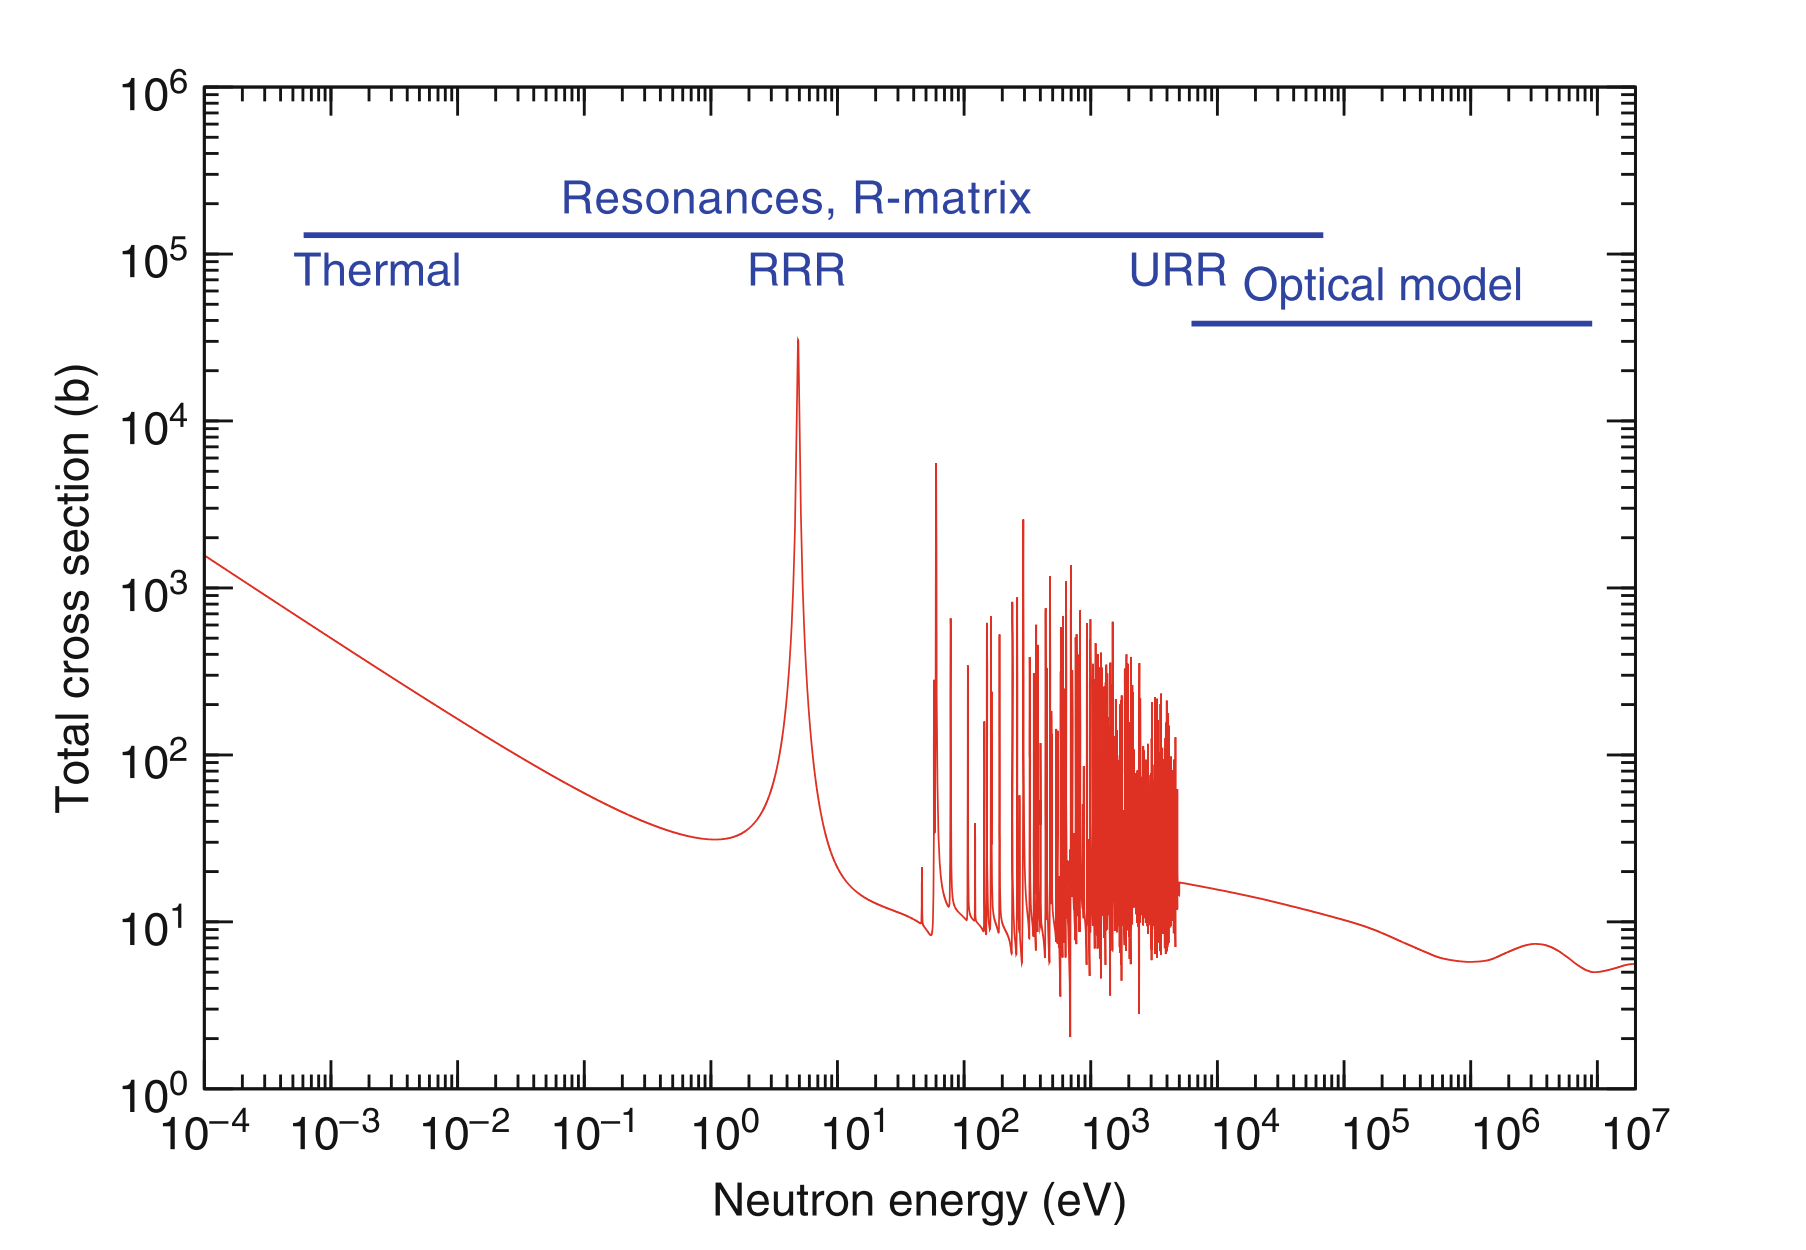
\includegraphics[width=\textwidth]{au-197_sigma_tot}
  \caption{The total cross-section as a function of energy for \textsuperscript{197}Au. Note the smooth $1/v$ region where the probability of interaction decreases with energy (interactions are more likely to happen with greater time). Subsequently, resonances are the dominant phenomenon from eV--keV energies. As the level density increases past the energy resolution achievable in experiments, the RRR becomes the URR. Past this, a continuum region is obtained and methods other than resonance theory must be used to predict behaviour. Figure from \cite{Cacuci2010}.}
  \label{fig:au-197_sigma_tot}
\end{figure}

\subsection{Probability tables}
\label{subsec:prob_table}
% njoy2016 pg. 635 is a detailed description of generation - very helpful
As stated above, in the URR individual resonances cannot be discerned. However, by applying the appropriate nuclear reaction theory, it is possible to determine the probable values for various resonance parameters in the URR region. These include the probability distribution for the spacings (Wigner distribution) and distributions for the partial widths ($\chi^{2}$ distributions for various degrees of freedom) \cite{MacFarlane2016}. An ENDF type evaluation may give these at various energies through the URR and different nuclear spins. This information can be used to generate Probability Tables (PTs). This concept was developed in the 1970s by Levitt, Nikolaev et al. Here the PDF as a function of energy for the total cross-section and conditional probabilities for indiviudal reaction channels can be given. Several codes are capable of producing these PTs, including NJOY \cite{MacFarlane2010} and CALENDF \cite{sublet2017b}. These codes use a Monte Carlo approach for generating the PTs, first sampling a starting resonance, then sampling partial widths for that resonance, before sampling for the next resonance. This is continued to build a `resonance ladder'. A series of these ladders are generated, with greater numbers converging to physical results \cite{Brown2017}. 

\nomenclature[z]{PT}{Probability Table}

\subsection{Cross-sections}
As explored above, it is beneficial to encode the cross-sections of resonant reactions in a parameterised way. Compared with a simple list of ($\sigma$, E) tuples it is more insightful and permits the reconstruction of cross-sections from resonance data for different material temperatures. However, past a certain point, resonances overlap because the aforementioned average resonance widths become much greater than the average level spacing, i.e. $\left<\Gamma\right> \gg \left<D\right>$ and so the combined, overlapping resonances form a continuum (see figure~\ref{fig:au-197_sigma_tot}). Any scheme based on describing individual resonances is no longer practical. 

For this high energy range then, where cross-sections change relatively slowly as a function of energy, simple tabulated data is used. This data can be obtained experimentally and with the aid of theoretical frameworks such as the `optical' model and Hauser Feshbach theory \cite{Hauser1952}. This cross-section information is recorded in MF=3 with a single MT for each open reaction channel. For instance, MF=3, MT=102 is \textsuperscript{i}X(n,$\gamma$)\textsuperscript{i+1}X for nuclide \textsuperscript{i}X. Where cross-sections reconstructed from resonance parameters do not match experimentally measured totals, corrections are also recorded here.

\subsection{Differential distributions}
Both energy and angular distributions are important for the accurate simulation of radiation transport through matter. For simple interactions such as elastic scattering, the scattered angle and energy of a particular interaction can be calculated kinematically if the particle masses and incident energy are known. Repeating this process for a population of particles at low energies, one can deduce that elastic scattering is isotropic. However, nuclear reactions are not necessarily isotropic in the distribution of their products. Especially for direct nuclear reactions, where the energy is high, emitted particles may be forward biased. This is because at high energies, the wavelength of an incident particle is similar to the size of the scattering nucleus and so diffraction occurs. As with a light wave diffracting around a sphere, there is a peak directly behind the sphere. Forward biasing is of particular importance in fusion systems given the 14.1 MeV `birth' energy of D-T fusion neutrons. The angular distributions of nuclear reaction products can be well represented by Legendre polynomials. For higher energies, higher order Legendre polynomials are required. The Rodrigues formula for generating Legendre polynomials is shown below as equation~\ref{eq:rodrigues}. An example angular distribution for elastic scattering off \textsuperscript{186}W is shown as figure~\ref{fig:tungsten_scatter}.

\begin{equation}
  P_{n}(x) = \frac{1}{2^{n}n!} \frac{\mathrm{d}^{n}}{\mathrm{d}x^{n}} (x^{2} - 1)^{2}
  \label{eq:rodrigues}
\end{equation}

\begin{figure}[ht]
%  \figuretitle{}
  \centering
  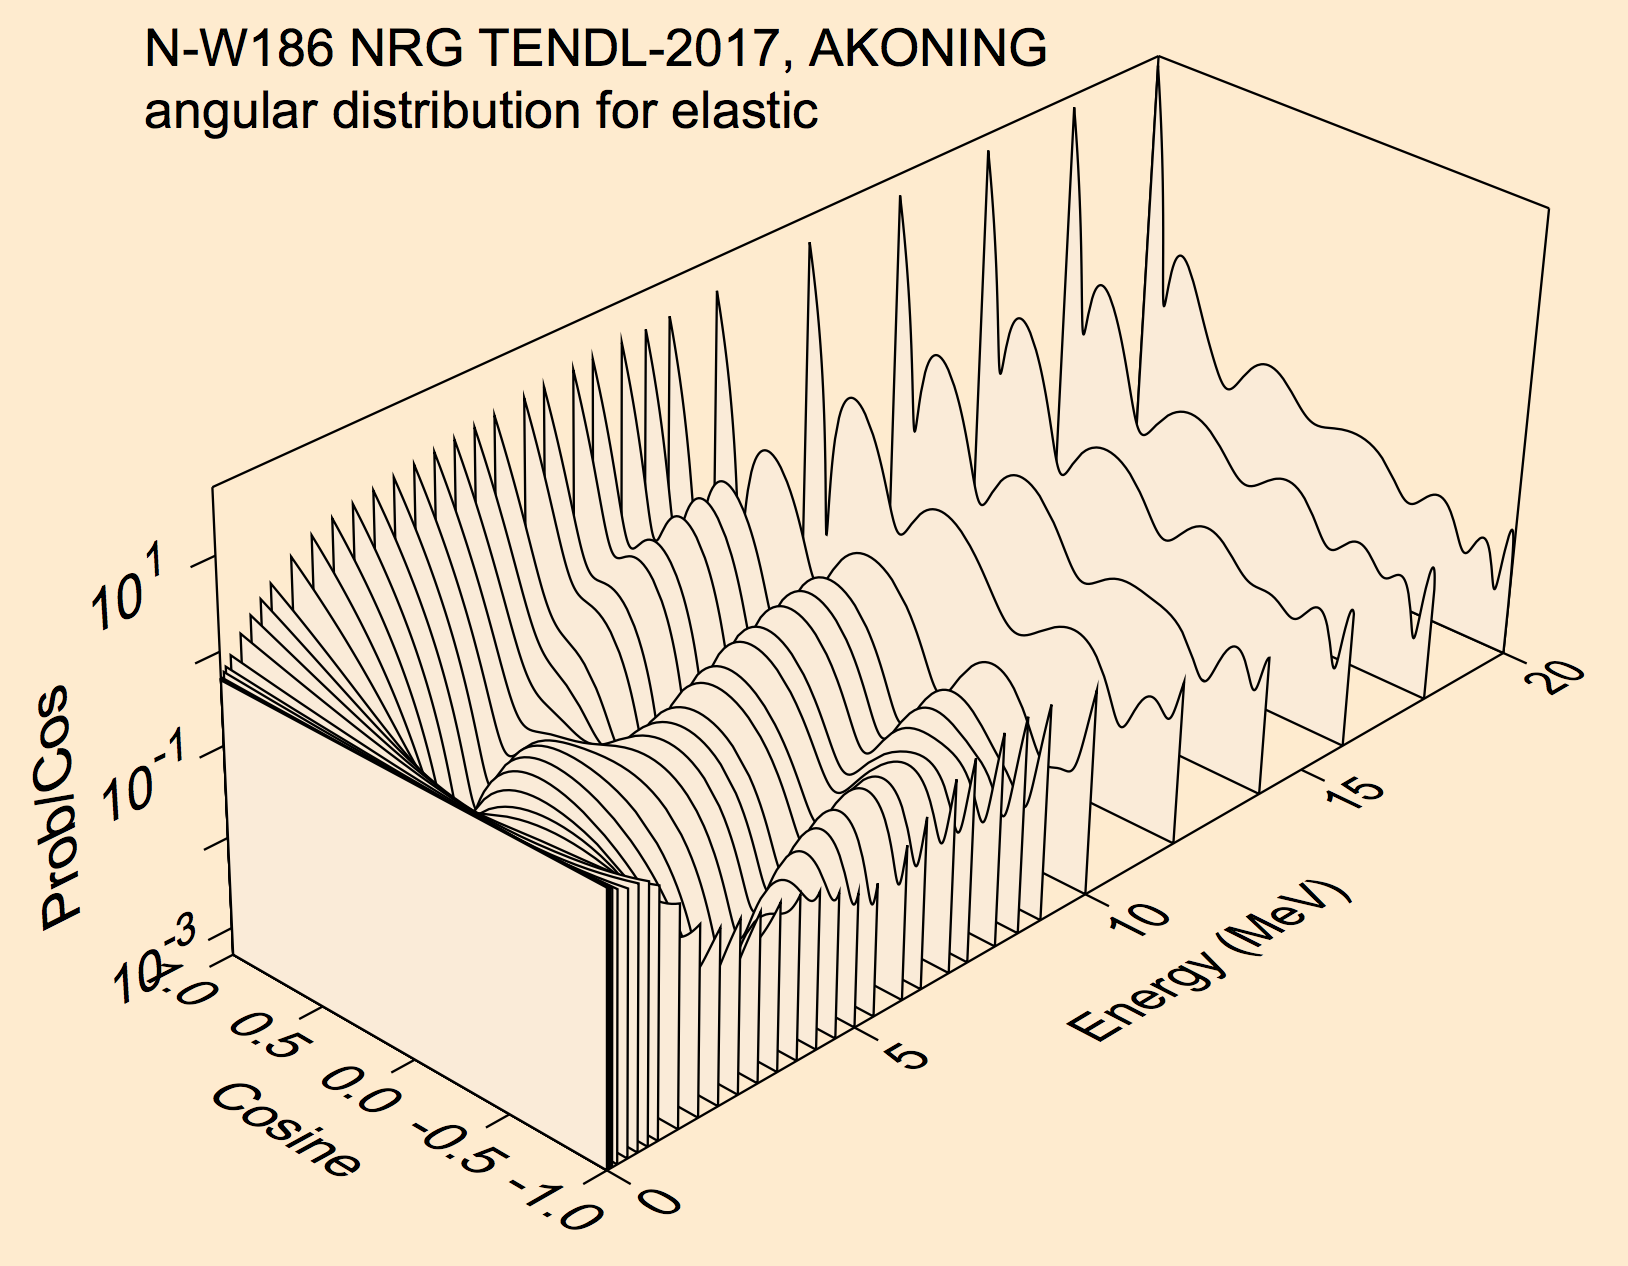
\includegraphics[width=0.7\textwidth]{tungsten_scatter}
  \caption{The angular distribution of elastically scattered neutrons off \textsuperscript{186}W. The probability is normalised by the cosine of the scattered angle. Note the isotropic nature at low energies, moving to a more anisotropic behaviour for greater energies. This plot was produced with NJOY \cite{MacFarlane2010} and released as part of the TENDL2017 library \cite{Rochman2016}.}
  \label{fig:tungsten_scatter}
\end{figure}

Energy and angular distributions are found in MF=4,5,6 depending on the age and type of evaluation.

\subsection{Decay}
Unstable nuclei decay, that is, change by the emission of particles or by internal conversion of one nucleon to another. Radionuclides may be primordial, that is, manufactured in stars and supernovae or activated/transmuted in the present, into radionuclides from a stable parent nuclide. The process of attaining stability through decay is also described by ND. Half-lives, $\gamma$-photon, and other particle emission probabilities, and energies are recorded along with fission product yield data in MF=8. 

\subsection{Covariances}
% ENDF-6 formats §29.1 very useful as overview material
% \cite{Rullhusen2006} may be helpful too!
Without information on uncertainty, data may be worse than just wrong, it may be falsely reassuring. The practical utility of some ND is in part determined by its uncertainty, whether its quoted value is likely to be near the true value. For uncertainties to be quoted with engineering results, uncertainty must first be quantified within the inputs (ND). Then, ND uncertainties can be propagated by various methods through to quantities of interest such as powers, neutron multiplication factors or material temperatues. The uncertainty data is a description of the experimental variance on certain data points, say, a cross-section for a given reaction channel and energy, but also with covariance information. These covariance data describe how correlated pairs of mean value data are. These correlations often arise from systematic measurement errors in nuclear physics experiments, where data for a whole energy range might be biased similarly in some way. The files containing variance and covariance information are colloquially known simply (and a little confusingly) as `covariances' or `covariance files'. Until recently, uncertainty information was only released in nuclear data library documentation or accompanying references. The modern ENDF-6 standard groups variance and covariance information together with the mean value data \cite{ENDF-6}. 

\section{Radiation transport methods}
\label{sec:radiation_transport}
% Boltzmann equation and intro
\subsection{Deterministic methods}
\label{subsec:deterministic}
% Brief overview, don't spend too long
\subsection{Stochastic methods}
\label{subsec:monte_carlo}
% Sampling not solving the Boltzmann equation, more involved description of MC

\section{Material activation-transmutation methods}
% Bateman equation and its solution
% pg 11-12 of below may be helpful
% https://fispact.ukaea.uk/wp-content/uploads/2016/06/FISPACT-II-introchapter1.pdf  

\section{Sources of uncertainty in fusion neutronics}
The sources of uncertainty in fusion neutronics are many and varied. Currently envisioned fusion reactors such as ITER rank as some of the most complex machines ever. Their multitude of components, diversity of materials and range of temporal and spatial scales make simulating their operation challenging. This complexity requires immense computational resources to model with a high fidelity. It is not currently possible to model any engineering system \textit{ab initio}, solving the Schr{\"o}dinger equation for each nucleon. Instead, approximations at each distance and time scale are made and fidelity traded off against simulation time. Examples of various modelling approximations commonly employed in fusion neutronics analyses follow below. These practices enable the solution of otherwise insoluble problems.  

\begin{itemize}
\item Omission of material impurities. These are important for calculating expected activation of materials.
\item Omission of small components. If mass is not conserved this could be deleterious for shielding analyses.
\item Omission of fluid flow. Important for modelling $\gamma$ dose from $^{16}$N generated in water cooling systems.
\item Spatial homogenisation of complex geometries. This very common practice combines adjacent volumes of differing materials to a mixture. When done correctly, mass will be conserved. However, the new homogenised materials alter the neutron spectrum and therefore the nuclear responses.
\item Discretisation of the spatial domain. When particle fields and associated nuclear responses are computed using a stochastic, Monte Carlo approach, there is no functional description and instead the results are binned spatially. The bin resolution has an impact on the result. 
\item Discretisation of the particle energy domain. This can result in so-called self-shielding errors as discussed in a later chapter, the coarser the energy binning the more potentially erroneous the result.
\item Assuming temporal invariance of plasma neutron source. This neglects the variability of plasma neutron emission from turblence and other plasma physics effects.
\item Assuming temporal invariance of material compositions. While some studies explicitly model material changes, others do not due to the additional complexity and computational burden involved.
\item Assuming plasma neutron source axisymmetry. This is despite notable toroidal heterogeneity due to neutral beam on thermal plasma interactions.
\item No multiphysics feedback with thermal processes. Example processes include Doppler broadening of materials' neutron cross-sections and thermalisation of neutron spectra.
\end{itemize}

Design uncertainty is also \textit{de rigueur}, with large electricity producing plant several decades away. Neutronic analyses may take months to complete, during which time plant subassemblies designs' change, partially invalidating the analysis. 

While the devices themselves are large and difficult to model, introducing uncertainties into calculations, other kinds of uncertainty are inherent in the practice of neutronics, regardless of the resources available. The knowledge of nuclear physics, colloquially referred to as `nuclear data' (ND) \nomenclature[z]{ND}{Nuclear Data} is not precisely known for two main reasons. These are:  

\begin{itemize}
  \item Uncertainty in experimentally derived data. These uncertainties can be energy specific as with poor statistics for certain energy bins, or more general, such as `normalisation uncertainties' like poor knowledge of sample mass or target geometry.
  \item Uncertainty in nuclear physics model parameters. Where experimental data does not exist, theoretical models are used to estimate nuclear behaviour. These models require input parameters that can are either experimentally measured themselves--with some uncertainty--or are interpolated or extrapolated from other experimental information. 
\end{itemize}

% Now explain the size of some of these uncertainies
Our incomplete knowledge of nuclear physics coupled with limited computing power and complex, interrelated systems means many nuclear processes in controlled fusion cannot be simulated precisely. Instead they are approximated with the help of heuristics and simplifications as outlined above. Sometimes the degree of certainty in a result is quantified, but often, especially where Monte Carlo methods are used, the uncertainty of some result is not given, as it is detached from uncertainty in its input parameters.

\section{Implications of current uncertainties}
The current engineering and physics uncertainties have a potentially large impact on realising fusion electricity. 

\subsection{Tritium breeding}
To give an example, the amount of tritium consumed by a fusion power plant would be approximately 55.6kg FPY$^{-1}$ GW$^{-1}$ \nomenclature[z]{FPY}{Full Power Year}. Depending on the design, the uncertainty on the Tritium Breeding Ratio (TBR) \nomenclature[z]{TBR}{Tritium Breeding Ratio} may be between 8\% and 18\% \cite{El-Guebaly2009}. For a plant with $P_{fus}=3\mathrm{GW}$ \nomenclature[a]{$P_{fus}$}{Fusion power} this results in between $\pm7.6$ kg and $\pm15$kg uncertainty on tritium production when running at full power for a year. These are very large quantities of tritium, for comparison total world production in Heavy Water Reactors (HWRs) \nomenclature[z]{HWR}{Heavy Water Reactor} is currently 4 kg y$^{-1}$ \cite{Kovari2018}. Underproducing tritium has the potential to rapidly curtail the operation of future fusion plant and to make it very difficult to provide a start-up inventory for subsequent devices. Overproducing is not ideal either, with regulatory agencies staunchly opposed to large stockpiles of tritium within the plant, given its danger as a highly permeable, radioactive gas with a function in nuclear weapons. Therefore reducing the uncertainty on TBR values and producing the exact amount required is highly desirable.

\subsection{Cost of fusion electricity}
Currently the Cost of Electricity (CoE) \nomenclature[z]{CoE}{Cost of Electricity} from future fusion plants is expected to be be approximated by equation~\ref{eq:coe}. 

\begin{equation}
  \label{eq:coe}
  CoE \propto \left(\frac{rF}{A}\right)^{0.6} \frac{1}{\eta^{0.5}_{th} P^{0.4}_{e} \beta^{0.4}_{N} N^{0.3}}
\end{equation}

Where $r$ is the discount rate, $F$ the learning factor, $A$ the plant availability, $P_{e}$ the electrical power generated, $\beta_{N}$ the normalised $\beta$ and $N$ the multiplier of the density compared to the density limit scaling. The cost of fuel is not an important factor, rather the capital cost as influenced by certain engineering parameters, the availability and the cost of money (interest) as represented by the discount rate. See \cite{Ward2005} for further explanation of equation~\ref{eq:coe}. The most expensive systems to construct in fusion power plants will be, in descending order, the magnets, the buildings / civil engineering work and the blanket assemblies \cite{Entler2018}. A large degree of uncertainty in the nuclear responses relevant for these systems will result in increased costs through unnecessarily conservative shielding and the risk of reduced component lifetimes (thus lowering availability to facilitate early replacements). 

It is worth drawing a parallel between the fission and future fusion experiences of regulation. The cost of nuclear fission reactors in countries such as the USA and France has increased over time \cite{Lovering2016}. Studies have associated between 14\% and 21.5\% of cost increases with an increase in regulatory activity from the domestic nuclear regulatory agency \cite{Cantor1988}. It seems unlikely that nuclear regulation will decrease in stringency in the future. Given this, uncertainty in the nuclear responses such as neutron and photon dose to workers, long-lived radioactive material production, tritium generation and nuclear heating of magnets will likely increase costs further by drawing the attention of regulators.

%\subsection{Magnet longevity}
% Potential third section, uncertainty on fluence / nuclear heating in TFC

The above discussion has provided a series of motivations for quantifying and reducing the uncertainty currently encountered in the nuclear analyses of fusion systems.

% Current capital cost estimates, especially given plant cost (and the interest on that cost) is the main driver of CoE
% Current plant complexity
% Regulatory considerations, compare operation to fission
% TBR deficit for DEMO
% Shielding of electronics in ITER

\section{Thesis outline}
This introductory chapter has described the motivations for the development of controlled nuclear fusion energy. There was a discussion of the historical development of our nuclear physics understanding and the engineering development of magnetic confinement fusion. Following this, a breif review of radiation-matter interactions and their relevance. Some examples of uncertain phenomena in fusion technology were given, along with their implications for the realisation of a fusion power plant. 

% TMC
The next chapter is an exploration of Total Monte Carlo (TMC) \nomenclature[z]{TMC}{Total Monte Carlo} applied to TBR simulations. Starting with a review of ND forms, this piece of work identifies potential contributions to TBR uncertainty and attempts to estimate the uncertainty due to lead nuclear data. The results highlight the capability of TMC in determining the distribution of uncertainty and how distribution skewness should be considered an important factor in risk analysis.

% Spatial homogenisation
Chapter 3 details an investigation into the practice of spatial homogenisation for radiation transport. First, a review of relevant literature is presented. Then, homogenisation within the ITER reinforced concrete bioshield is used to determine how significantly this approximation diverges from physical behaviour. Estimates of over and under-estimates of dose to workers are given for on-load and shut-down (activated) scenarios. Finally, advice on the appropriateness of this practice is given for various shielding scenarios and further work recommended.

% Group structure optimisation
Chapter 4 describes the development and testing of an algorithm to optimise the discretisation of the energy domain for activation and transmutation calculations. It begins with a discussion of relevant nuclear physics, developing an understanding of nuclear resonances and their distribution in the $\{E, Z, A\}$ space of interaction energy, nucleus proton number and mass. This information is used to develop a method for the targeting of energy resolution where it is most valuable. A series of tests are presented where optimised and logarithmically spaced Multi-Group (MG) \nomenclature[z]{MG}{Multi-Group} results are compared with Point-Wise (PW) \nomenclature[z]{PW}{Point-Wise} Reaction Rate (RR) \nomenclature[z]{RR}{Reaction Rate} values. Opportunities for improvement and further testing of the algorithm are presented.

% Drawing conclusions
The final chapter draws conclusions on the implications of the previously discussed sources of uncertainty. Their interrelated and compounded nature is discussed along with recommended future work in this area.

